\documentclass[12pt]{article}
\usepackage{setspace,graphicx,amsmath,geometry,fontspec,titlesec,soul,bm,subfigure}
\titleformat{\section}[block]{\LARGE\bfseries}{\arabic{section}}{1em}{}[]
\titleformat{\subsection}[block]{\Large\bfseries\mdseries}{\arabic{section}.\arabic{subsection}}{1em}{}[]
\titleformat{\subsubsection}[block]{\normalsize\bfseries}{\arabic{subsection}-\alph{subsubsection}}{1em}{}[]
\titleformat{\paragraph}[block]{\small\bfseries}{[\arabic{paragraph}]}{1em}{}[]
\setmainfont{Times New Roman}
\renewcommand{\baselinestretch}{1.15}
\renewcommand\contentsname{Inhaltverzeichnis}
\geometry{a4paper,left=2.5cm,right=2.5cm,top=2.5cm,bottom=2.5cm}
\begin{document}
	\newpagestyle{main}{            
		\sethead{}{Kapitel 2}{} 
		\setfoot{}{\thepage}{}
		\headrule
		\footrule
			}
	\pagestyle{main}
\tableofcontents
\newpage
\section{Ingenieurgeodätische Netze}
\subsection{Punktvermarkung}
\subsection{Netzdimension und Koordinatensysteme}
\textbf{Netzdimension: 1, 2 oder 3 Dimensionen.}
\newline
\newline
\textbf{Eindimensionale Netze} = Höhennetze. z.B DHHN oder lokales Netz.
\newline
Messmethoden: Nivellement und Gravimetrie. altenativ: GNSS und Geoidhöhen oder andere speziale Verfahren.
\newline
Datumfestlegung: 1 Verschiebung (Festlegung des Nullpunktes)
\newline
Historische Aufbau in Deutschland
\begin{table}[ht]
\begin{tabular}{ll}
1.Ordnung: & Schleifen Durchmesser 30 - 80 km \\
2.Ordnung: & Schleifen Durchmesser 20 km \\
3.Ordnung: & Schleifen Durchmesser 10 km\\
4.Ordnung: & Schleifen Durchmesser < 4 km
\end{tabular}
\end{table}
\newline
\textbf{Zweidimensionale Netze} = Lagenetze z.B UTM, Gauß-Krüger, lokale Netze, DHDN.
\newline
Messmethoden: Winkel + Strecken oder GNSS.
\newline
Datumfestlegung: 2 Verschiebungen, 1 Rotation, 1 Maßstab. 
Historische Aufbau in Deutschland
\begin{table}[ht]
	\begin{tabular}{ll}
		1.Ordnung: & Punktabstand 30 - 40 km \\
		2.Ordnung: & Punktabstand 10 - 20 km \\
		3.Ordnung: & Punktabstand 3 - 10 km\\
		4.Ordnung: & Punktabstand 1 - 3 km
	\end{tabular}
\end{table}
Verdichtung durch Aufnahmepunkte / Polygonpunkte.
\newline
\newline
\textbf{Dreidimensionale Netze} z.B WGS 84, ITRF 2008 ...
\newline
Messmethoden: 
\newline
GNSS, VLBI, SLR, DORIS (global)
\newline
Winkel und Strecken (lokal)
\newline
Datumfestlegung: 3 Verschiebungen, 3 Rotationen, 1 Maßstab.
\subsection{Netzqualität}
- Definition der Netzqualität (Netzgüte) durch Qualitätsmerkmale.
\newline
- Qualitätsparameter (Gütekriterien) konkretisieren die Qualitätsmerkmale.
\newline
Beispiel: Genauigkeit ist ein Qualitätsmerkmal, aber Beschreibung durch den numerischen Wert für einen Parameter z.B Standardabweichung.
\newline
- Qualitätsmerkmale Ingenieurgeodätischer Netze:
\begin{itemize}
\item Genauigkeit
\item Zuverlässigkeit (Kontrollierbarkeit)
\item Sensitioität (Empfindlichkeit gegenüber Deformation)
\item Seeperabilität / Trennbarkeit (von Deformationsmodellen)
\end{itemize}
Qualitätsparameter werden zur Netzoptimierung hergezogen. d.h. Optimierung von funktionalen und/oder Stochastischen Modell um z.B Spur zu minimieren. 
\subsubsection{Genauigkeit}
Grundlagen: Kovarianzmatrix der Parameter/Koordinaten (m ist die Anzahl der Punkte)
\begin{equation*}
\bm{\Sigma}_{\hat{x}\hat{x}} = \sigma_0^2 \cdot \bm{Q}_{\hat{x}\hat{x}} = 
\begin{bmatrix}
\bm{\Sigma}_{11} & \bm{\Sigma}_{12} & \cdots \\
\bm{\Sigma}_{21} & \ddots      & \vdots \\
\cdots & \cdots & \bm{\Sigma}_{mm}
\end{bmatrix} \quad 
mit\ \ \bm{\Sigma}_{ii} = \begin{bmatrix}
\sigma_x^2 & \sigma_{xy} \\
\sigma_{xy} & \sigma_y^2 \\
\end{bmatrix} \quad  i = 1,2,\cdots, m
\end{equation*}
\paragraph{lokale Genauigkeitsmaße}
\noindent A.Punktbezogen, absolute
\newline
A1. Helmert'sche Punktfehler
\begin{equation*}
\sigma_{H,i} = \sqrt{\sigma_x^2 + \sigma_y^2} \quad (= \sqrt{spur(\bm{\Sigma}_{ii})})
\end{equation*}
Varianzkriterium: $\sigma_{H,i} \Rightarrow min$
\newline
A2. Punktfehler nach Werkmeister
\begin{equation*}
\sigma_{W,i} = \sqrt{det({\bm{\Sigma}_{ii})}}
\end{equation*}
Volumenkriterium: $\sigma_{W,i} \Rightarrow min$
\newline
Forderung: Ellipsoidfläche möglichst klein
\begin{gather*}
F = A_1 \cdot A_2 \cdot \pi \\
F^2 = A_1^2 \cdot A_2^2 \cdot \pi^2 \\
F^2 = \sigma_0^4 \cdot \pi^2 \cdot (\xi_{2,1-\alpha}^2)^2 \cdot \lambda_1 \cdot \lambda_2 \\
\sigma_0^4 \cdot \pi^2 \cdot (\xi_{2,1-\alpha}^2)^2\ \ ist\  Konstant\  und\ \ \  \lambda_1 \cdot \lambda_2 = det(\bm{\Sigma}_{ii})
\end{gather*}
A2 hat den Vorteil, dass auch die Kovarianz $\sigma_{xy}$ berücksichtigt wird.
\newpage
\noindent A3. Eigenwertkriterium.
\begin{figure*}[ht]\centering
\subfigure[Problem F1 = F2]{
	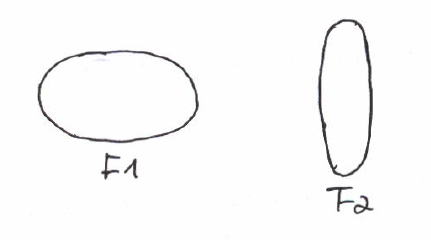
\includegraphics[width=0.3\textwidth]{2-2Ellipse.png}}
\end{figure*}
\begin{equation*}
\frac{\lambda_{max}}{\lambda_{min}} \Rightarrow 1 \quad oder \quad \lambda_{max} \Rightarrow \lambda_{min} \quad allgemein \ ideal
\end{equation*}
B.Relative Genauigkeitsmaße
\newline
$\Rightarrow$ bezogen auf Koordinatendifferenzen.\newline
$\Rightarrow$ wichtig für Nachbarschaftsgenauigkeit\newline
Relative Standardabweichungen
\begin{gather*}
\Delta_{\hat{x}_{i,j}} = \Delta_{\hat{x}_{i}} - \Delta_{\hat{x}_{j}} \\
\sigma_{\Delta \hat{x}_{i,j}} = \sqrt{\sigma_{\hat{x}_i}^2 + \sigma_{\hat{x}_j}^2 - 2 \sigma_{\hat{x}_{i,j}}}
\end{gather*}
Relative Sub-Kovarianzmatrix
\begin{equation*}
\bm{\Sigma}_{\Delta_{lk}} = \bm{\Sigma}_{ll} + \bm{\Sigma}_{kk} - \bm{\Sigma}_{kl} - \bm{\Sigma}_{lk}
\end{equation*}
A1 bis A3 dann auf B anwendbar.
\paragraph{Globale Genauigkeitsmaße}
\noindent Gesamte $\Sigma_{\hat{x}\hat{x}}$ wird verwendet, gesamtes Netz wird beurteilt. \newline
Erweitertes Varianzkriterium
\begin{equation*}
spur(\bm{\Sigma}_{\hat{x}\hat{x}}) \Rightarrow min
\end{equation*}
Erweitertes Volumenkriterium
\begin{equation*}
det(\bm{\Sigma}_{\hat{x}\hat{x}}) \Rightarrow min
\end{equation*}
"Darstellung" als Konfidenzhyperellipsoid.\newline
Erweiterte Eigenwertkriterium
\begin{equation*}
\frac{\lambda_{max}}{\lambda_{min}} \Rightarrow 1 \quad oder \quad \lambda_{max} \Rightarrow \lambda_{min} 
\end{equation*}
Eigenwertkriterium ist besonders sinnvoll, da jede beliebige Funktion der Parameter minimiert wird.
\begin{gather*}
\bm{\hat{\chi}} \ \ ist \ eine\  beliebige \ Funktion \\
\varphi(\bm{\hat{\chi}}) = \bm{f} \cdot \bm{\hat{\chi}} \\
\sigma_{\varphi}^2 = \bm{f} \bm{\Sigma}_{\hat{x}\hat{x}} \bm{f^{T}}
\end{gather*}
Es gilt $\bm{f^T} \bm{f} \lambda_{max} \geq \sigma_{\varphi}^2 \geq \bm{f^T} \bm{f} \lambda_{min} \longrightarrow \lambda_{min} \leq \frac{\sigma_{\varphi}^2}{\bm{f^T} \bm{f}} \leq  \lambda_{max}\quad$ (Releigh-Relation). \newline
Eigenwertkriterium führt auch zu Minimierung des Varianz einer beliebigen Netzfunktion.\newline
\textbf{Hauptkomponenten Analysis} \newline
1.Hk: (u ist die Anzahl der Unbekannter)
\begin{equation*}
\bf{P_1} = \bf{s_1} \cdot \sqrt{\lambda_1} = \begin{bmatrix}
s_{11} \\
s_{12} \\ 
\vdots \\
s_{1u}
\end{bmatrix} \cdot \lambda_1
\end{equation*} 
2.Hk: 
\begin{equation*}
\bf{P_2} = \bf{s_2} \cdot \sqrt{\lambda_2}
\end{equation*}
\begin{equation*}
\vdots \quad \vdots \quad \vdots
\end{equation*}
mit $\lambda_1 = maximaler\ Eigenwert$ und $\lambda_1 \geq \lambda_2 \geq \cdots$. \newline
\newline
- Funktion, die in Richtung $\bm{s_1}$ wirkt, ist am ungenausten bestimmt.\newline
- Um so größer der Anteil von $\bm{P_1}$ an Gesamtvarianz, um so größer der Effekt von $\lambda_1$ (bis zu $60\%$ möglich, dann "wesentliche Eigenvektoren")\newline
- Jede Koordinate des Netzes wird durch den Eigenvektor ein Varianzanteil zugeordnet. Dadurch wird an jedem Punkt der am schwächsten bestimmte Richtung definiert.\newline
\textbf{Homogenität} \newline
Alle Konfidenzellipsen bzw. -ellipsoide weisen die selbe Struktur auf, alle $A_1$ sind gleichlang, alle $A_2$ gleichlang ...\newline
\textbf{Homogenität und Isotropie} \newline
Alle Konfidenzellipsen bzw. -ellipsoide sind Kreis- bzw. kugelförmig. Alle Halbachse gleichlang.\newline
\textbf{Vollständige Isotropie} \newline
Isotropie gilt auch für relative Konfidenzellipsen, Radian der Kreise/Kugeln können zwischen punktbezogenen und relativen Kreise/Kugeln unterschiedlich ausfallen.
\newpage
\paragraph{Vergleich verschiedener Messverfahren}
\noindent Genetzte numerische Werte 
\begin{align*}
&Entfernungsmessung(EDM) &\sigma_D^2 = (2mm)^2 + (1,5ppm)^2 \\
&Richtung  &\sigma_r = 0,25mgon \Rightarrow \sigma_q = D \cdot \sigma_r\\
&GNSS &\sigma_b^2 = (3mm)^2 + (0,5ppm)^2 \\
\end{align*}
wobei
\begin{align*}
& \sigma_D \Rightarrow Strecknmessgenauigkeit \\
& \sigma_r \Rightarrow Richtungsmessgenauigkeit \\
& \sigma_b \Rightarrow Basisliniengenauigkeit (GNSS) 
\end{align*}
Bitte Werte je nach Verfahren und Instrumenten einsetzen! 
\begin{table}[ht]\centering
	\begin{tabular}{|l|l|l|l|}
		\hline
		$D[m]$ & $\sigma_D[mm]$     &   $\sigma_q[mm]$   &  $\sigma_b [mm]$   \\ \hline
		100      & 2,0  & 0,4  & 3,0 \\ \hline
		200      & 2,0  & 0,8  & 3,0 \\ \hline
		500      & 2,1  & 2,0  & 3,0 \\ \hline
		700      & 2,2  & 2,7  & 3,0 \\ \hline
		1000     & 2,5  & 3,9  & 3,0 \\ \hline
		2000     & 3,6  & 7,9  & 3,2 \\ \hline
		5000     & 7,8  & 19,6 & 3,9 \\ \hline
		10000    & 15,1 & 39,3 & 5,8 \\ \hline
	\end{tabular}
\end{table}
Optimaler Punktabstand für kombinierte Richtungs- und Streckenmessung ca. 400 bis 600 m  
\subsubsection{Zuverlässigkeit}
In der Geodäsie: Kontrollierbarkeit = Aufdeckbarkeit von Fehlern durch geometrischen Überbestimmung.(Fehler können im stochastischen und im funktionalen Modell möglich sein.)
\begin{equation*}
\bm{Q_{vv}} = \bm{Q_{ll}} - \bm{Q_{\hat{l}\hat{l}}}
\end{equation*}
mit
\begin{equation*}
\bm{Q_{\hat{l}\hat{l}}} = \bm{A} \cdot \bm{Q_{\hat{x}\hat{x}}} \bm{A^T}
\end{equation*}
\paragraph{Innere Zuverlässigkeit}
\noindent Global:\newline 
Freiheitsgrad(Reudanz der Ausgleichung) 
\begin{gather*}
f = n - u + d \\
f = spur(\bm{Q_{vv}} \cdot \bm{P}),\\
\bm{Q_{vv}} \cdot \bm{P} \ \ ist Redudanzmatrix
\end{gather*}
Bedingungsdichte: (relativer Wert zur Übereinstimmung)
\begin{equation*}
b = \frac{r}{n} = \frac{f}{n} \quad mit \  1 \geq b \geq 0
\end{equation*}
bei $b = 0(f \neq 0)$:keine Übereinstimmung, $b = 1$: alle Beobachtungen $100 \%$ konktrolliert(nicht möglich)
Lokal: \newline
bezogen auf Beobachtungen
\begin{gather*}
\bm{v} = -\bm{Q_{vv}} \cdot \bm{P} \cdot \bm{l}
\end{gather*}
Annahme: Fehler in Beobachtung $l_i$: $\Delta l_i$
\begin{gather*}
\bm{v} = -\bm{Q_{vv}} \cdot \bm{P} \cdot (\bar{\bm{l}} + \bm{Q_i} \Delta l_i)\\
\bar{\bm{l}}\ \ ist\ \ fehlerfreie\  \ Vektor \\
\bm{l} = \begin{bmatrix}
0\\
0\\
0\\
\vdots \\
1\\
\vdots\\
0\\
0\\
0\\
\end{bmatrix} \\
\bm{v} = \bar{\bm{v}} - \bm{Q_{vv}} \cdot \bm{P} \cdot \bm{L_i} \cdot \Delta l_i\\
\Delta l_i \ \ betrachtet\ \  als\ \  globaler\ \  Fehler.
\end{gather*}
Auswirkung des groben Fehlers:
\begin{equation*}
\Delta v_i = -(\bm{Q_{vv}} \cdot \bm{P})_{ii} \cdot \Delta l_i = -r_i \cdot \Delta l_i
\end{equation*}
$\Delta l_i$ wirkt sich auf alle Verbesserungen aus. $\Rightarrow$ Verschmiereffekt.\newline
Redudanzanteil
\begin{equation*}
r_i = (\bm{Q_{vv}} \cdot \bm{P})_{ii}
\end{equation*}
$r_i$ sollte möglichst groß sein, um Verschmiereffekt klein zu halten: $r_i \rightarrow max$
\begin{equation*}
0 \leq r_i \leq 1 
\end{equation*}
\begin{align*}
\rightarrow & 1 \ \ theoretisch\  nicht\  zu\  erreichen.\\
\rightarrow &0\ \ ist\  ohne\  Kontrolle\\
\rightarrow &\leq 0,3 \ sollte\  vermieden\  werden \\
\rightarrow &0,5 \ \ als\ Ziel
\end{align*}
\begin{equation*}
f = r = \sum_{i = 1}^{n} r_i = \sum_{i = 1}^{n} (\bm{Q_{vv}} \cdot \bm{P})_{ii} = spur(\bm{Q_{vv}} \cdot \bm{P}) = rang(\bm{Q_{vv}} \cdot \bm{P})
\end{equation*}
Beispiel (Redudanz 2D)
\begin{figure*}[ht]\centering
	\subfigure[]{
		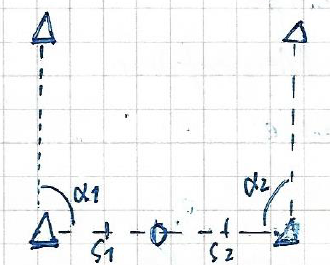
\includegraphics[width=0.4\textwidth]{Innerzuverlaessigkeit_beispiel.png}}
\end{figure*}
\begin{table}[ht]\centering
	\begin{tabular}{|l|l|l|}
		\hline
	Beobachtungen & Redudanz     &   Redudanzanteile      \\ \hline
		$\alpha_1,s_1$      & 0  & 0   0   \\ \hline
		$\alpha_1, s_1, s_2$     & 1  & 0   0,5   0,5  \\ \hline
		$\alpha_1, \alpha_2, s_1, s_2$      & 2  & 0,5   0,5   0,5   0,5   \\ \hline
	\end{tabular}
\end{table}
\newline
Minimal aufdeckbarer Beobatungsfehler $\nabla l_i^2$ \newline
Nichtzentralitätsparameter
\begin{equation*}
\delta_i = \frac{\Delta l_i^2 \cdot p_i^2 \cdot q_{vv,i}}{\sigma_0^2} \Leftrightarrow \Delta l_i^2 = \frac{\delta_i \cdot \sigma_0^2}{p_i^2 \cdot q_{vv,i}}
\end{equation*}
$\longrightarrow$ Übergang auf Grenzwert $\delta_0$
\begin{align*}
\nabla l_i = & \sigma_0 \cdot \sqrt{\frac{\delta_0}{p_i^2 \cdot q_{vv,i}}} \\
=& \sigma_0 \cdot \sqrt{\frac{\delta_0}{p_i \cdot r_i}} \\
=& \sigma_i \cdot \sqrt{\frac{\delta_0}{r_i}} \quad mit \quad  \sigma_i = \sigma_0 \frac{\delta_0}{r_i}
\end{align*}
Dieser Wert gibt an, wie groß ein Beobachtungsfehler werden muss, um mit anschließenden Test aufgedeckt zu werden.
\begin{equation*}
\nabla l_i \longrightarrow min
\end{equation*}
Häufige Forderung
\begin{equation*}
\nabla l_i ~ (6\ bis \ 8)\ \sigma_i
\end{equation*}
\paragraph{Äußere Zuverlässigkeitsmaße}
\noindent Null
\paragraph{Vergleich verschiedenen Messverfahren}
\noindent anhand der Bedingungsdichte 
a. Streckennetz
\begin{figure*}[ht]\centering
	\subfigure[Strekennetz: 4 Diagonalenvierecke]{
		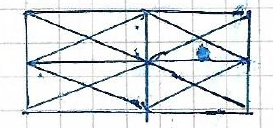
\includegraphics[width=0.4\textwidth]{strecken.png}}
\end{figure*}
\begin{gather*}
n = 20\\
v = 2 \times 9 = 18\\
d = 3\\
f = 20 - 18 + 3 = 15\\
b = \frac{f}{n} = 0,25
\end{gather*}
b. Winkelnetz
\begin{figure*}[ht]\centering
	\subfigure[1 diagonal]{
		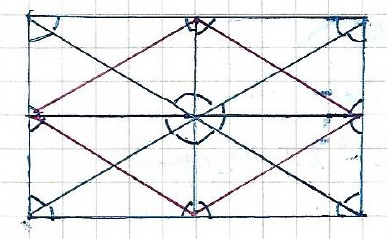
\includegraphics[width=0.4\textwidth]{winkel.png}}
	\subfigure[2 diagonal]{
		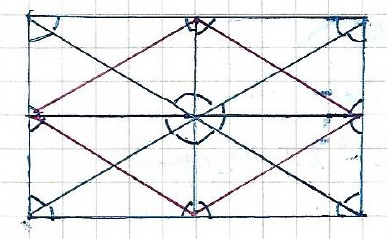
\includegraphics[width=0.4\textwidth]{winkel.png}}
\end{figure*}
\newline
b1. eine Diagonale pro Viereck
\begin{gather*}
n = 18(Aussenwinkel) + 5(Innenwinkel)\quad da\ Summe\ der\ Winkeln\ immer\ 400\ gon\\
n = 23\\
v = 18\\
d = 4\\
f = 9\\
b = \frac{9}{23} = 0,39
\end{gather*}
b2. zwei Diagonale pro Viereck
\begin{gather*}
n = 24 + 7 = 31\\
f = 31 - 18 + 4 = 17\\
b = \frac{17}{31} = 0,55
\end{gather*}
c. kombinierte Netze \newline
Diagonal Vierecke mit Strecken und Winkeln(a + b2)
\begin{gather*}
n = 31(Winkeln) + 20(Strecken) = 51 \\
v = 18\\
d = 3\\
f = 36 \\
b = \frac{36}{51} = 0,71
\end{gather*}
In der Realität: 0,5 bis 0,6 \newline
d. Polygonzug als negative Beispiel(beideseitig angeschlossen)(obwohl kombiniertes Netz)
\begin{gather*}
f = 3\\
b = \frac{b}{n} = \frac{3}{n} = \frac{3}{v + 3}
\end{gather*}
\begin{table}[ht]\centering
	\begin{tabular}{|l|l|l|}
		\hline
		Punktanzahl & v     &   b      \\ \hline
		1      & 2  & 0,6   \\ \hline
		2      & 4  & 0,43  \\ \hline
		3      & 6  & 0,33   \\ \hline
		4      & 8  & 0,27  \\ \hline
		5      & 10  & 0,23   \\ \hline
	\end{tabular}
\end{table}
\newline
e.Lagenetz mit GNSS
\begin{figure*}[ht]\centering
	\subfigure[GNSS]{
		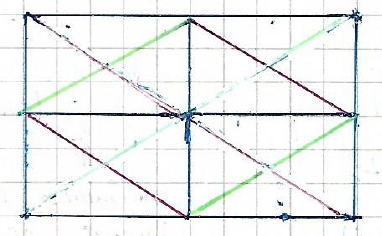
\includegraphics[width=0.4\textwidth]{GNSS.png}}
\end{figure*}
\newline
e1.(blau) (12 Beobachtungen $\longrightarrow$ 24 Koordinaten) \newline
e2.(blau,rot) (16 Beobachtungen, 32 Koordinaten) \newline
e3.(blau,rot,grün) (20 Beobachtungen, 40 Koordinaten) \newline
$v=18, d=2$, da Rotation und Maßstab gemessen
\begin{table}[ht]\centering
	\begin{tabular}{|l|l|l|l|}
		\hline
	          &  e1     &   e2    & e3  \\ \hline
		b     & 8  & 16  & 24 \\ \hline
		f     & 0,33  & 0,5 & 0,6\\ \hline
	\end{tabular}
\end{table}
\begin{itemize}
\item GNSS und kombiertes Netz bringen vergleichbare gute Ergebnisse
\item Strckennetz und insbesondere Polygonzug fallen deutlich ab
\item Winkelnetz erfordert hohen Aufwand um mit GNSS oder Kombinationslösung zu konkurrieren.
\end{itemize}
\subsection{Datumsdefinition}
\begin{equation*}
r_Q = v - d
\end{equation*}
Durch Beobachtung der Datumsparameter kann der Datumdefekt reduziert werden. Die Kompensation kann verhindert werden, wenn die entsprechende Parameter geschätzt wird, deshalb muss diese Möglichkeit nicht genutzt werden (z.B Maßstabsschätzung trotz Streckenmessung)
\subsection{Datumsverfügung}
\subsubsection{Einfügung}
Datumsverfügung kann geschehen durch \newline
a. Nutzung von Festpunkte \newline
$\longrightarrow$ hierachische Ausgleichung, Normalgleichungsmatrix $\bm{N}$ ist regulär und invertierbar. \newline
b. Nutzung von Datumpunkte \newline
freie Ausgleichung \newline
$\longrightarrow$ Normalgleichungsmatrix $\bm{N}$ ist singulär und nicht invertierbar.(Pseude-inverse nötig) \newline
Bei singuläre Matrix $\bm{N}$ benötigt man Ränderungsmatrizen $\bm{G}$
\begin{equation*}
\begin{bmatrix}
\bm{N} & \bm{G} \\
\bm{G^T} & \bm{0}
\end{bmatrix}^{-1} = \begin{bmatrix}
\bm{N}^+ & \bm{G} \\
\bm{G^T} & \bm{0}
\end{bmatrix}
\end{equation*}
Im Prinzip ist $\bm{G}$ freiwählbar und muss nur den Rangabfall ausgeglichen.
\begin{align*}
\bm{N}:& \quad zu\ invertierende\ Matrix \\
\bm{G}:& \quad Raenderungsmatrix \\
\bm{N}^+ :& \quad Moor-Penrose-Inverse/Pseude\ Inverse
\end{align*}
Forderung:
\begin{gather*}
\bm{N}\cdot \bm{G} = \bm{0}\\
\bm{G}^T \bm{\hat{x}} = \bm{0}(zusaetzlich)
\end{gather*}
Dimension von $\bm{G}$: $u \times d$, $u$ ist Anzahl der Unbekannter, $d$ ist Anzahl der Datumdefekt.\newline
Alternative Rängderungsmatrix über Spektralzerlegung:
\begin{gather*}
\bm{N} = \bm{S} \cdot \bm{D} \cdot \bm{S}^T\\
\bm{D}: Spektralmatrix \\
\bm{S}^T: Modelmatrix\ mit\ Eigenvektoren\\
\bm{S} = (\bm{S_r},\bm{S_0})\\
dim(\bm{S_r}) = q,r_Q\\
dim(\bm{S_0}) = q,d
\end{gather*}
$\bm{S_0}=\bm{G}$: normierte Ränderungsmatrix.\newline
Allgemeine Ränderungsmatrizen $\bm{B}$ über sogenannten Helmertbedingungen.
\begin{equation*}
g_{ij} = \frac{b_{ij}}{\sqrt{\sum_{i = 1}^{u}b_{ij}^2}},\quad j = 1,2,\cdots, d
\end{equation*}
Überführung von $\bm{B}$ nach $\bm{G}$.\newline
Ableitung von $\bm{G}$ aus $\bm{B}$ für 1D-Fall
\begin{equation*}
\bm{G} = \begin{bmatrix}
\frac{1}{\sqrt{u}}\\
\frac{1}{\sqrt{u}}\\
\ddots\\
\frac{1}{\sqrt{u}}\\
\end{bmatrix}, da\ \sum b_i^2 = u
\end{equation*}
Gesamtspurminimierung: \newline
$\longrightarrow$ Alle Punkte tragen zur Datumfestlegung bei.\newline
Inversion
\begin{equation*}
\bm{N}^+ = (\bm{N} + \bm{G}\bm{G}^T)^{-1} - \bm{G}\bm{G}^T
\end{equation*}
außerdem:$\hat{x}$ mit minimalem Norm, $\hat{x}^T\hat{x} \longrightarrow min$ \newline
Teilspurminimierung\newline
$\rightarrow$ Nur ein Teil der Punkte tragen zur Datumfestlegung bei.
\begin{gather*}
\bm{G_i} = \bm{E_i}\bm{G} \\
\bm{E_i} = \begin{bmatrix}
\bm{I_p} & \bm{0} \\
\bm{0} & \bm{0}
\end{bmatrix}\quad (Auswahlmatrix)
\end{gather*}
$I_p$ hat Dimension der Anzahl der Datumfestliegende Koordinaten $p$
\begin{equation*}
\bm{G_i} = \bm{E_i}\bm{G} = \begin{bmatrix}
\bm{G_p} \\
\bm{0}
\end{bmatrix}
\end{equation*}
Inversion:
\begin{equation*}
\begin{bmatrix}
\bm{N} & \bm{G_i}\\
\bm{G_i^T} & \bm{0}
\end{bmatrix}^{-1} = \begin{bmatrix}
\bm{N}^{-1} & \bm{G(G_i^T G)}^{-1}\\
(\bm{G^T G_i})^{-1} \bm{G^T} & \bm{0}
\end{bmatrix}
\end{equation*}
$\bm{N}^{-1}$ ist generalsierte Inverse von $\bm{N}$ mit minimaler Teilspur für $p$ Koordinaten und minimaler Norm für $p$ Koordinaten.
\begin{equation*}
\bm{N}^{-1} = (\bm{N + G_i G_i^T})^{-1} - \bm{G(G_i^T G)}^{-1} \bm{(G^T G_i)}^{-1} \bm{G^T}
\end{equation*}
Übergang zur Gesamtspurminimierung\newline
Es gilt $\bm{G^T G} = \bm{I}$ und es wird $\bm{E_i} = \bm{I}$ und $\bm{G_i} = \bm{G}$
\begin{align*}
\bm{N}^- =& (\bm{N} + \bm{G G^T})^{-1} - \bm{G}(\bm{G^T G})^{-1}(\bm{G^T G})^{-1} \bm{G^T}\\
= & (\bm{N} + \bm{G G^T})^{-1} - \bm{G}\bm{G^T}\\
= & \bm{N^{+}}
\end{align*}
Übergang zur zwangsfreien Netz mit $p=d\rightarrow \bm{N}^{-} = \bm{N}^{+} \rightarrow \bm{\hat{x}^T \hat{x}}$ wird Null.
\subsection{Datumstransformationen}
\subsubsection{Allgemeines}
\subsubsection{Kombination von terrestrischen und GNSS messungen}
Generelle Vorgehensweise 3D Datumsübergang.
\begin{itemize}
\item $\bm{{x}}$: Koordinatensystem "GNSS" (WGS 84)
\item $\bar{{{\bm{x}}}}$: Landeskoordinatensystem(ETRS 89)
\end{itemize}
\begin{gather*}
\bm{x} = \bm{x_0} + (1 + m) \bm{R} \bar{\bm{x}} \quad Transformationsgleichung\\
\bm{x_0} = \begin{bmatrix}
x_0 \\
y_0\\
z_0\\
\end{bmatrix} \quad Translationen \\
\bm{R} = \begin{bmatrix}
1 & \varepsilon_z & -\varepsilon_y \\
-\varepsilon_z & 1 &  \varepsilon_x \\
\varepsilon_y & - \varepsilon_x & 1
\end{bmatrix} \quad Rotationsmatrix\ mit \ den\ Rotationen\ \varepsilon_x,\ \varepsilon_y,\ \varepsilon_z \\
m:\quad Massstab \\
\Longrightarrow 7 \ Parametern: m,x_0,y_0,z_0,\varepsilon_x,\varepsilon_y,\varepsilon_z
\end{gather*}
Bestimmung der Datumsparameter. \newline
für Punkt $i$:
\begin{align*}
x_i = & x_0 + (1 + m)(\bar{x}_i + \varepsilon_z \cdot \bar{y}_i - \varepsilon_y \cdot \bar{z}_i)\\
y_i = & x_0 + (1 + m)(-\varepsilon_z \cdot \bar{x}_i + \bar{y}_i + \varepsilon_x \cdot \bar{z}_i) \\
z_i = & x_0 + (1 + m)(\varepsilon_y \cdot \bar{x}_i - \varepsilon_x \cdot \bar{y}_i + \bar{z}_i)
\end{align*} 
\begin{align*}
{x_i} = & {x}_0 + \bar{{x}_i} + \varepsilon_z \cdot \bar{{y}_i} - \varepsilon_y \cdot \bar{{z}_i} + m \cdot \bar{{x}_i} + m \cdot  (\varepsilon_z \cdot \bar{{y}_i} - \varepsilon_y \cdot \bar{{z}_i}) \\
\approx & {x}_0 + \bar{{x}_i} + \varepsilon_z \cdot \bar{{y}_i} - \varepsilon_y \cdot \bar{{z}_i} + m \cdot \bar{{x}_i} \quad (fuer\  kleine\  Drehwinkel)
\end{align*}
$\Longrightarrow$ Gauß-Markov-Modell einsetzen!
\begin{gather*}
\Delta x_i = (x_i - \bar{x}_i) = x_0 + \varepsilon_z \bar{y}_i - \varepsilon_y \bar{z}_i + m \bar{x}_i \\
\begin{bmatrix}
\Delta x_1 \\
\Delta y_1 \\
\Delta z_1 \\
\vdots \\
\Delta x_m \\
\Delta y_m \\
\Delta z_m \\
\end{bmatrix} = \begin{bmatrix}
1 & 0 & 0 & \bar{x}_1 & 0 & -\bar{z}_1 & \bar{y}_1 \\
0 & 1 & 0 & \bar{y}_1 & \bar{z}_1 & 0 & -\bar{x}_1 \\
0 & 0 & 1 & \bar{z}_1 & -\bar{y}_1 & \bar{x}_1 & 0 \\
\vdots & \vdots & \vdots & \vdots & \vdots & \vdots & \vdots \\
1 & 0 & 0 & \bar{x}_m & 0 & -\bar{z}_m & \bar{y}_m \\
0 & 1 & 0 & \bar{y}_m & \bar{z}_m & 0 & -\bar{x}_m \\
0 & 0 & 1 & \bar{z}_m & -\bar{y}_m & \bar{x}_m & 0 \\
\end{bmatrix} \cdot \begin{bmatrix}
x_0 \\
y_0 \\
z_0 \\
m \\
\varepsilon_x \\
\varepsilon_y \\
\varepsilon_z
\end{bmatrix}
\end{gather*}
Häufiges Problem: \newline
Stochastisches Modell
\begin{equation*}
\bm{\sum_{\Delta x \Delta x}} = \bm{\sum_{xx}} + \bm{\sum_{\bar{x} \bar{x}}}
\end{equation*}
\begin{itemize}
\item $\bm{\sum_{xx}}$ häufig optimistisch, oft nicht $100 \%$ verfügbar.
\item $\bm{\sum_{\bar{x} \bar{x}}}$ aus historische Gründe oft nicht komplett vorhanden.(Abschätzung erforderlich!)
\end{itemize}
\end{document}